%% BioMed_Central_Tex_Template_v1.06
%%                                      %
%  bmc_article.tex            ver: 1.06 %
%                                       %

%%IMPORTANT: do not delete the first line of this template
%%It must be present to enable the BMC Submission system to
%%recognise this template!!

%%%%%%%%%%%%%%%%%%%%%%%%%%%%%%%%%%%%%%%%%
%%                                     %%
%%  LaTeX template for BioMed Central  %%
%%     journal article submissions     %%
%%                                     %%
%%          <8 June 2012>              %%
%%                                     %%
%%                                     %%
%%%%%%%%%%%%%%%%%%%%%%%%%%%%%%%%%%%%%%%%%


%%%%%%%%%%%%%%%%%%%%%%%%%%%%%%%%%%%%%%%%%%%%%%%%%%%%%%%%%%%%%%%%%%%%%
%%                                                                 %%
%% For instructions on how to fill out this Tex template           %%
%% document please refer to Readme.html and the instructions for   %%
%% authors page on the biomed central website                      %%
%% http://www.biomedcentral.com/info/authors/                      %%
%%                                                                 %%
%% Please do not use \input{...} to include other tex files.       %%
%% Submit your LaTeX manuscript as one .tex document.              %%
%%                                                                 %%
%% All additional figures and files should be attached             %%
%% separately and not embedded in the \TeX\ document itself.       %%
%%                                                                 %%
%% BioMed Central currently use the MikTex distribution of         %%
%% TeX for Windows) of TeX and LaTeX.  This is available from      %%
%% http://www.miktex.org                                           %%
%%                                                                 %%
%%%%%%%%%%%%%%%%%%%%%%%%%%%%%%%%%%%%%%%%%%%%%%%%%%%%%%%%%%%%%%%%%%%%%

%%% additional documentclass options:
%  [doublespacing]
%  [linenumbers]   - put the line numbers on margins

%%% loading packages, author definitions

\documentclass[twocolumn]{bmcart}% uncomment this for twocolumn layout and comment line below
%\documentclass{bmcart}

%%% Load packages
%\usepackage{amsthm,amsmath}
%\RequirePackage{natbib}
%\RequirePackage{hyperref}
\usepackage[utf8]{inputenc} %unicode support
%\usepackage[applemac]{inputenc} %applemac support if unicode package fails
%\usepackage[latin1]{inputenc} %UNIX support if unicode package fails

% % %My package
\usepackage{graphicx}
\usepackage{pifont} 



%%%%%%%%%%%%%%%%%%%%%%%%%%%%%%%%%%%%%%%%%%%%%%%%%
%%                                             %%
%%  If you wish to display your graphics for   %%
%%  your own use using includegraphic or       %%
%%  includegraphics, then comment out the      %%
%%  following two lines of code.               %%
%%  NB: These line *must* be included when     %%
%%  submitting to BMC.                         %%
%%  All figure files must be submitted as      %%
%%  separate graphics through the BMC          %%
%%  submission process, not included in the    %%
%%  submitted article.                         %%
%%                                             %%
%%%%%%%%%%%%%%%%%%%%%%%%%%%%%%%%%%%%%%%%%%%%%%%%%


%\def\includegraphic{}
%\def\includegraphics{}
  

%%% Put your definitions there:
\startlocaldefs
\endlocaldefs


%%% Begin ...
\begin{document}

%%% Start of article front matter
\begin{frontmatter}

\begin{fmbox}
\dochead{Research}

%%%%%%%%%%%%%%%%%%%%%%%%%%%%%%%%%%%%%%%%%%%%%%
%%                                          %%
%% Enter the title of your article here     %%
%%                                          %%
%%%%%%%%%%%%%%%%%%%%%%%%%%%%%%%%%%%%%%%%%%%%%%

\title{Evaluation of Multiple Features for \\
	Violent Scene Detection}

%%%%%%%%%%%%%%%%%%%%%%%%%%%%%%%%%%%%%%%%%%%%%%
%%                                          %%
%% Enter the authors here                   %%
%%                                          %%
%% Specify information, if available,       %%
%% in the form:                             %%
%%   <key>={<id1>,<id2>}                    %%
%%   <key>=                                 %%
%% Comment or delete the keys which are     %%
%% not used. Repeat \author command as much %%
%% as required.                             %%
%%                                          %%
%%%%%%%%%%%%%%%%%%%%%%%%%%%%%%%%%%%%%%%%%%%%%%

\author[
   addressref={aff1},                   % id's of addresses, e.g. %{aff1,aff2}
   %corref={aff1},                       % id of corresponding address, if %any
   %noteref={n1},                        % id's of article notes, if any
   email={lqvu@fit.hcmus.edu.vn}   % email address
]{\inits{VL}\fnm{Vu} \snm{Lam}}
\author[
   addressref={aff2},
   email={plsang@nii.ac.jp}
]{\inits{SP}\fnm{Sang} \snm{Phan}}
\author[
addressref={aff2},
email={ledduy@nii.ac.jp}
]{\inits{DL}\fnm{Duy-Dinh} \snm{Le}}
\author[
addressref={aff3},
email={ducda@uit.edu.vn}
]{\inits{DD}\fnm{Duc Anh} \snm{Duong}}
\author[
addressref={aff2},
email={satoh@nii.ac.jp}
]{\inits{SS}\fnm{Shin'ichi} \snm{Satoh}}

%%%%%%%%%%%%%%%%%%%%%%%%%%%%%%%%%%%%%%%%%%%%%%
%%                                          %%
%% Enter the authors' addresses here        %%
%%                                          %%
%% Repeat \address commands as much as      %%
%% required.                                %%
%%                                          %%
%%%%%%%%%%%%%%%%%%%%%%%%%%%%%%%%%%%%%%%%%%%%%%

\address[id=aff1]{%                           % unique id
  \orgname{University of Science}, % university, etc
  \street{227 Nguyen Van Cu, Dist. 5},                     %
  %\postcode{}                                % post or zip code
  \city{Ho Chi Minh},                              % city
  \cny{Vietnam}                                    % country
}
\address[id=aff2]{%
  \orgname{National Institute of Informatics},
  \street{2-1-2 Hitotsubashi, Chiyoda-ku},
  \postcode{101-8430}
  \city{Tokyo},
  \cny{Japan}
}
\address[id=aff3]{%
	\orgname{University of Information Technology},
	\street{Quarter 6, Linh Trung Ward, Thu Duc District},
%	\postcode{101-8430}
	\city{Ho Chi Minh},
	\cny{Vietnam}
}
%\address[id=aff4]{%
%	\orgname{The Graduate University for Advanced Studies (SOKENDAI)},
%	\street{Shonan Village, Hayama, Kanagawa},
%	\postcode{240-0193}
%%	\city{Ho Chi Minh},
%	\cny{Japan}
%}
%%%%%%%%%%%%%%%%%%%%%%%%%%%%%%%%%%%%%%%%%%%%%%
%%                                          %%
%% Enter short notes here                   %%
%%                                          %%
%% Short notes will be after addresses      %%
%% on first page.                           %%
%%                                          %%
%%%%%%%%%%%%%%%%%%%%%%%%%%%%%%%%%%%%%%%%%%%%%%

\begin{artnotes}
%\note{Sample of title note}     % note to the article
%\note[id=n1]{Equal contributor} % note, connected to author
\end{artnotes}

%\end{fmbox}% comment this for two column layout

%%%%%%%%%%%%%%%%%%%%%%%%%%%%%%%%%%%%%%%%%%%%%%
%%                                          %%
%% The Abstract begins here                 %%
%%                                          %%
%% Please refer to the Instructions for     %%
%% authors on http://www.biomedcentral.com  %%
%% and include the section headings         %%
%% accordingly for your article type.       %%
%%                                          %%
%%%%%%%%%%%%%%%%%%%%%%%%%%%%%%%%%%%%%%%%%%%%%%

\begin{abstractbox}

\begin{abstract} % abstract
	Violent scene detection (VSD) is a challenging problem because of the heterogeneous content, large variations in video quality, high semantic meaning of the concepts. In the last few years, combining multiple features from multi-modalities is proven as an effective strategy for a wide range of general multimedia event detection (MED), but the specific event detection like VSD has been comparatively less studied. In this work, we evaluate the value of multi features and combination of these features in a violent scene detection system. We rigorously analyze and combine a set of low-level features and deep learning feature that capture appearance, color, texture, motion and audio in videos. We also evaluate the utility of mid-level visual information obtained from detecting related violent concepts. Experiments are performed on MediaEval VSD 2014 dataset, which are made publicly available. Results show the performance of visual and motion features are better than audio features. The performance of mid-level features was nearly as good as that of low-level visual features. Experiments with a number of fusion methods show that all single features are complementary and help to improve overall performance. This study also provides an empirical foundation for selecting feature sets that are capable of dealing with heterogeneous content data as violent scenes in movies.
\end{abstract}

%%%%%%%%%%%%%%%%%%%%%%%%%%%%%%%%%%%%%%%%%%%%%%
%%                                          %%
%% The keywords begin here                  %%
%%                                          %%
%% Put each keyword in separate \kwd{}.     %%
%%                                          %%
%%%%%%%%%%%%%%%%%%%%%%%%%%%%%%%%%%%%%%%%%%%%%%

\begin{keyword}
\kwd{violent scene detection}
\kwd{video retrieval}
\kwd{multi-modal fusion}
\kwd{multiple features}
\end{keyword}

% MSC classifications codes, if any
%\begin{keyword}[class=AMS]
%\kwd[Primary ]{}
%\kwd{}
%\kwd[; secondary ]{}
%\end{keyword}

\end{abstractbox}
%
\end{fmbox}% uncomment this for twcolumn layout

\end{frontmatter}

%%%%%%%%%%%%%%%%%%%%%%%%%%%%%%%%%%%%%%%%%%%%%%
%%                                          %%
%% The Main Body begins here                %%
%%                                          %%
%% Please refer to the instructions for     %%
%% authors on:                              %%
%% http://www.biomedcentral.com/info/authors%%
%% and include the section headings         %%
%% accordingly for your article type.       %%
%%                                          %%
%% See the Results and Discussion section   %%
%% for details on how to create sub-sections%%
%%                                          %%
%% use \cite{...} to cite references        %%
%%  \cite{koon} and                         %%
%%  \cite{oreg,khar,zvai,xjon,schn,pond}    %%
%%  \nocite{smith,marg,hunn,advi,koha,mouse}%%
%%                                          %%
%%%%%%%%%%%%%%%%%%%%%%%%%%%%%%%%%%%%%%%%%%%%%%

%%%%%%%%%%%%%%%%%%%%%%%%% start of article main body
% <put your article body there>

%%%%%%%%%%%%%%%%
%% Background %%
%%


\section{Introduction}

\begin{figure*}
	\centering
	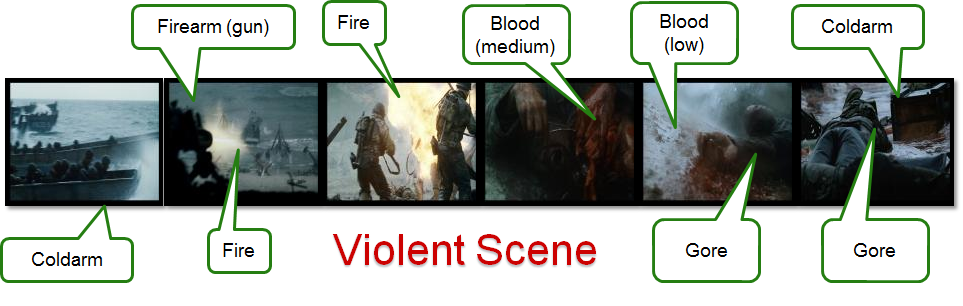
\includegraphics[width=2\linewidth]{Images/ViolentScene.png}
	\caption{Following the violent definition in \cite{demarty2014benchmarking}, this is an example of a violent scene in Saving Private Ryan Movie because it contains physical violence or accident resulting (fighting scene: boats approaching, guns shooting, fire guns shooting,..) in human injury or pain (blood and gory, dead soldiers)}
	\label{fig:exampleVS}
\end{figure*}

Nowadays, the movie industry generates thousands of movies each year. However, not all movies are suitable for young people (especially children, teenagers, e.g.) to watch, because they might have violent contents.   The research from University of Pittsburgh \cite{TVMovieViolence} reports that watching violence in movies or TV programs tends to make children more aggressive and leads to unhealthy attitudes. It is crucial to have violent scene detection (VSD) system which enables the parents to choose movies that are suitable for their children. More general, for content provider, the violent scene detection technique can be used to assist in movie rating; for general end users, it can block the violent content in client terminal devices. 

Given a movie as input, the expected output of a VSD system is all shots having violent information. A general framework \cite{demarty2014benchmarking,myers2014evaluating,oh2014multimedia} contains four main processing steps: video segmentation, feature extraction, learning models, and prediction. In the first step, the input movie is divided into fundamental processing units i.e. video shots. Then, features are extracted from the shots in second step. The goal of this step is to extract meaningful features which will be used for learning and predicting violence concept in shots in later steps. Related studies for similar system (e.g. multimedia event detection, action recognition, scene classification) have shown that selecting relevant features is essential for accurate detection.
\begin{figure*}
	\centering
	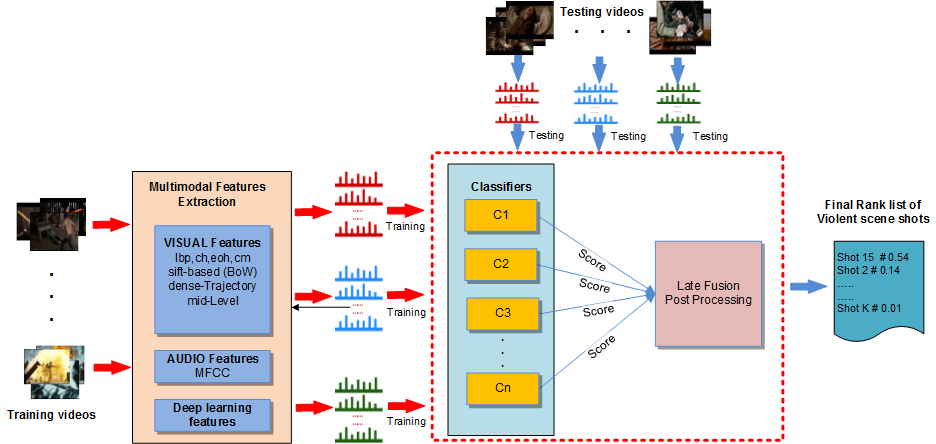
\includegraphics[width=2\linewidth]{Images/Framework1.png}
	\caption{Overview of violent scene detection framework.}
	\label{fig:framework}
\end{figure*}

%Detecting violent scene is a challenging task mainly due to the large variation of violence concept and the semantic gap between the concept and low-level features provided in the media. 
In this paper, we focus on the feature extraction step, we evaluate various types of features and their combinations especially for VSD. To capture violence insights, multiple features \cite{demarty2014benchmarking} (e.g. global or local static visual features, motion-based features, and audio features) are extracted for learning and prediction. Besides, to narrow the semantic gap \cite{SemanticGap}, a set of various mid-level concepts \cite{Concepts} and their spatial temporal relationships are used to characterize violence e.g. {\bf object-based concepts}: blood,  gun, cold arm, firearm; {\bf action-based concepts}: fighting, running, shooting, etc.; {\bf activity-based concepts}: car chase, boat chase; {\bf scene-based concepts}: gory scene, overcast, scene; {\bf sound-based concepts} such as gun shot, scream, explosion. Figure~\ref{fig:exampleVS} demonstrate an example of violent scene in a Hollywood movie. Specifically, we evaluate the following features in our VSD system:
\begin{figure*}[!t]
	\centering
	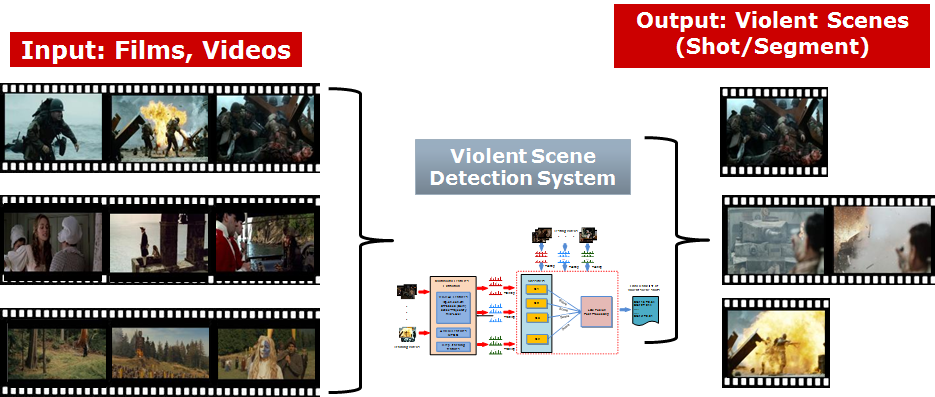
\includegraphics[width=2\linewidth]{Images/SystemOverview.png}
	\caption{Overview of violent scene detection system.}
	\label{fig:systemoverview}
\end{figure*}

\begin{itemize}
	\item {\bf Visual features.} We select following features for evaluation: color moments, color histogram, edge orientation histogram, and local binary patterns, SIFT, Color-SIFT, Opponent-SIFT ~\cite{burghouts2009performance}. Visual features are expected to be able to convey visual characteristics of the original violence concept, the object-based concepts, and the scene-based concepts.
	\item {\bf Audio feature.} We use the standard MFCC \cite{rabiner2007introduction} as audio feature. It is used for capturing specific sound signals in violent scenes to discriminate them from non-violent scenes (e.g. sounds of gun shots, a scream, or explosions). 
	\item {\bf Motion features.} in the movies, there are a lot of action with different movie effects in the violent	scenes. Motion feature	is one of the best approaches for action classification \cite{wang2013action}. We employ improved Dense Trajectory \cite{wang2013action} feature with Motion Boundary Histogram (MBH), Histograms of Oriented Gradients (HoG), and Histograms of Optical Flow (HoF) as features in presentation of action-based and activity-based concepts. This is to take the advantages of videos compared to static images.  
	\item {\bf Mid-level based feature.} To narrow the semantic gap, we use mid-level features to describe the original violence concept. Scores from classifiers of mid-level concepts are composed to form a unified feature for each shot. We then use these features for shot classification.
	\item {\bf Deep learning feature.} We also evaluate the performance of deep learning features due to its recent success on various image classification tasks \cite{krizhevsky2012imagenet}. We use the DeepCaffe \cite{jia2014caffe} framework for extracting deep learning feature. Outputs obtained from the last three layers are used to represent features of each shot. 
\end{itemize}
The main focus is to provide a comparative analysis on features and their contributions to the final performance of a VSD system. The observation drawn from our work may be helpful to future works in the field.
\renewcommand{\thefootnote}{\roman{footnote}}
We perform our experiments on a standard benchmark dataset, MediaEval VSD 2014  \cite{demarty2014benchmarking}, which are made publicly available \footnote{http://www.technicolor.com/en/innovation/research-innovation/scientific-data-sharing/violent-scenes-dataset} . Our system is trained and tested on Hollywood movies within MediaEval VSD Dataset. MediaEval VSD official metric (MAP-mean average precision) is used for evaluation. By using standard dataset and evaluation protocol, the performance of our system can be fairly compared to those from other MediaEval VSD participants (without using external data).

Results show the performance of visual features are the best. Low-level visual features and motion feature play very important role when fusing all modalities. Audio and mid-level features are not good as low-level visual features but they are complementary to improve overall performance. Experiments with several fusion methods show that all single features are complementary and help to improve overall performance.

The rest of this paper is organized as follows. We review some related work in section 2. Section 3 introduces our system, our approaches for feature extraction, and detail of feature configurations, fusion methods. In section 4, we describe our features using in VSD system. The experimental results and their analysis will be in section 5, as well as the discussion and conclusion are described in the section 5 of this paper.
\section{Related Work}
Violent scene detection is a kind of multimedia event detection. Although combining multiple features from multi-modalities has been proven as an effective strategy for multimedia event detection, relatively few works have been proposed to apply these approaches for violent scene detection in video. The main reason is that the definition of violence is ambiguous. It is difficult to describe this high-level concept using mathematical formulation precisely. In general, the violence concept is not well-defined and recent approaches addressed the problem by their own definitions.

Some of the previous works applied different kind of visual features to detect flame, blood, explosion as the informative cues for violence. As a first approach in this field, Jeho et al.\cite{nam1998audio} propose an approach to recognize violent scenes in videos by detecting flame and blood, capturing the degree of motion activity, the soundtrack and characterization of sound effects of violent events. Meanwhile, Chen et al.\cite{2} decompose violent scene detection into action scene detection and bloody frame detection. Clarin et al.\cite{3} present a system which uses a Kohonen self-organizing map, which is for detecting skin and blood pixels in each frame, and motion intensity analysis to detect violent actions involving blood. More recently, Gong Yu et al.\cite{11} introduce a violence detector using low-level visual and auditory features and high-level audio effects to identify potential violent content in movies. Jian \cite{17} describe a weakly-supervised audio violence classifier combined using co-training with a motion, explosion and blood video classifier to detect violent scenes in movies. Penet et al.\cite{21} compared two modality fusion methods, namely Early Fusion and Late Fusion. Early Fusion concatenates features from both modalities before machine learning, while Late Fusion fuses probabilities of both modalities already calculated. They reported Late Fusion was superior to Early Fusion.

Beside low-level based approaches, violent scene detection is also a kind of high level recognition task. The major challenge is to deal with the gap of semantic meaning. In recent years, there are some approaches using attributes to narrow the semantic gap in high-level recognition task, such as object recognition using attributes, scene classification using attributes, action recognition using actions bank\cite{23}. Li et al.\cite{15} propose ”Object Bank” (OB), a new representation of natural images based on objects (using objects as attributes to describe scenes). Liu et al.\cite{18} use high-level semantic concepts, also called attributes, to represent human actions from videos and argue that attributes enable the construction of more descriptive models for human action recognition. Sasanand et al.\cite{23} present Action Bank”, a new high-level representation (kind of attributes) of video.  For VSD, Bodgan et al.\cite{13} rely on fusing mid-level concept predictions made using multi-layer perception classifiers to automatically localize the occurrence of violence within a video.  They proposed a frame-level violence prediction, applying a multi-layer perceptron in order to utilize these concepts. They put the first layer for the concept prediction, and the second layer for the violence prediction. In addition to those provided concepts, Tan et al.\cite{tan2013vireo} have utilized extra 42 violence concepts such as bomb and war from ConceptNet\cite{liu2004conceptnet}. ConceptNet is composed of nodes representing concepts in the form of words or short phrases with their relationships. On their system those extra concepts are trained using YouTube videos which are crawled additionally. 

In the last few years, MediaEval Violent Scene Detection affect Task is become popular, many state-of-the art systems have been developed and reported recently\cite{demarty2014benchmarking}. Most systems extract a large number of multimodal features from visual, audio signals and text.  The features include low-level features such as color histogram, edge of histogram, local binary pattern, SIFT based, Space-Time Interest Points (STIP), Histograms of Oriented Gradients (HoG), Histograms of Optical Flow (HoF), Motion Boundary Histograms (MBH), visual activity, MFCCs, trajectory-based features  (cite each team). Different state-of-the-art features encoding are used, such as Bag-of-Visual-Words representation, Fisher vector representations. In addition, some approaches use of pre-defined concept detectors like part-level attributes – FUDAN Team\cite{dai2013fudan}, mid-level concept description, with provided concepts from ConceptNet (e.g., punishment, victim, rape, etc) – VIREO team\cite{tan2013vireo}. The video shots are classified by using different machine learning techniques (Support Vector Machines (SVMs), k nearest neighbors (kNN), Bayesian Network). Multimodal integration is achieved via early fusion\cite{penet2013technicolor} and late fusion\cite{penet2013technicolor,sjoberg2013far,derbas2013lig,dai2013fudan} where score fusion is often used to combine scores independently computed from different subsets of features.

In this paper, we present a novel violent scene detection framework which is designed to incorporate many of the above-mentioned success principles in its architecture. In particular, our work incorporates novel developments into the system, which can be summarized into major contributions. First, our work developed and incorporated multi modal features at diverse granularities to evaluate the value of different types of features for VSD. Second, our work explores the use of mid-level concept features, which are detected based on low-level features, aiming to provide more semantic understanding capability into our system. Third, we present several approaches to learn fusion functions which combine violent scores (late fusion) to improve overall performance.
\section{VSD System}
\subsection{Framework Overview}

We use a unified framework to evaluate the performance of each feature as well as the performance of feature combination methods. The framework should be flexible so that we can easily test different kind of features. It also should be designed in a component-based manner so that we can evaluate each component separately while keeping other components intact. In this spirit, our framework can be decomposed into following components: (1) Pre-processing, (2) Feature Extraction, (3) Feature Encoding, (4) Feature Classification and (5) Feature Fusion. The detail of each component is described in the following sections. We especially focus on the feature extraction and encoding component. It is used to produce necessary features for this evaluation. An overview of our framework is shown in Figure \ref{fig:framework}.
\subsection{Pre-Processing}
%\subsection{Keyframe Extraction and Shot Pooling}

The pre-processing step prepares data for further processing at later components. At first, videos are resized to the width of 500 pixels, while the resized height is scaled relatively so that the aspect ratio is kept. Motion features are extracted from the resized videos. This simple processing technique significantly reduce the processing time and still does not affect the detection performance, as shown in \cite{aly2013axes} for multimedia event detection.

For image features, keyframes are sampled at five frame per second. We found this sampling technique a good trade off between time and accuracy, as also suggested in \cite{merler2012semantic}. After that, blank keyframes, which are often filled with single color, are removed because they do not contain informative feature.

For audio features, we only extract the audio channel from the original video. Since the scale of the video does not affect the audio information, we use the original video for audio extraction and save as audio files with standard WAV format. Audio features will be extracted from these audio files directly.

\subsection{Feature Extraction}
The feature extraction component aims to make a discriminative vector representation for each shot that is extracted from the pre-processing step. The extraction method depends on what type of feature will be used. To conduct a comprehensive evaluation of features for VSD, we support a large variety of features including global and local visual features. Global features capture the global statistics of each extracted shot. These statistics can be calculated directly from sub regions of a sampled frame and then concatenated to form the vector representation for that frame, before being aggregated to make the final representation for each shot. It is more complicated to calculate the feature vector representation for local features. The number of local features vary from frame to frame, therefore it requires a special encoding technique which will be described in \ref{feature_encoding}.

Besides global and local features, other features are also supported in our evaluation framework. Audio feature can be extracted from pre-defined temporal windows. Feature of each temporal window provide a local audio characteristic at that temporal location. Therefore, audio feature can be considered as a local feature and can be well-integrated into our feature extraction framework. Another feature that is also supported is mid-level feature, which is represented from violent concept detectors. We consider both the in-domain and out-domain concept detectors. For in-domain concepts, we use violence related attributes (blood, fire, fight, fire arm, cold arm, ...) to create mid-level features. With out-domain concepts, we use very general attributes (outside violence domain) from off-the-shelf datasets ~\cite{deng2009imagenet}. We also employ the state-of-the-art deep learning features which are extracted from a pre-trained model. The detail description of each feature is presented in Section \ref{vsd_feature}.

\subsection{Feature Encoding}
\label{feature_encoding}
\subsubsection{Bag-of-words Encoding}

%\subsection{Feature representation}
As for local features, we employed the popular bag-of-words (BOW) model to generate a fixed-length feature representation from its local descriptors. The model was first applied to represent text document as mentioned in \cite{harris1954distributional}. It was adopted to represent image by Csurka et al. \cite{csurka2004visual}. Its extension to motion and audio features is also straightforward as described in \cite{sivic2009efficient} and \cite{jiang2010columbia}. 

We follow the experiment setup in \cite{jiang2010representations} to implement our bag-of-words models. We fix the codebook size to 1,000 because we observe that in \cite{jiang2010representations} the performance does not significantly improve when the larger codebooks were used. On the other hand, smaller codebook can significantly reduce the computational time for feature encoding as well as feature learning. In order to train the codebook, we randomly select 1M local descriptors and cluster using the K-means algorithm. The local descriptors are assigned to each codeword in a soft-weighting manner \cite{jiang2007towards} to improve the discriminative of the encoded feature.
\begin{figure}[!h]
	\centering
	\includegraphics[width=1\linewidth]{Images/Bow.png}
	\caption{Bag of visual words.}
	\label{fig:bow}
\end{figure}

The main drawback of the bag-of-words model is that it does not incorporate spatial information. The simplest way to overcome this problem is to partition the image into sub-regions and encode local features in each region independently. After that feature from all regions are concatenated into a single feature vector. There are many ways to partition an image into sub-region. To this end, we follow \cite{jiang2010representations} and \cite{lazebnik2006beyond} to use 2 \ding{53} 2 and 1 \ding{53} 3 spatial configurations. We found that these spatial configurations a good trade-off between performance and computational cost due to the high dimensional feature vector.

\subsubsection{Fisher Vector Encoding}
\begin{figure*}
	\centering
	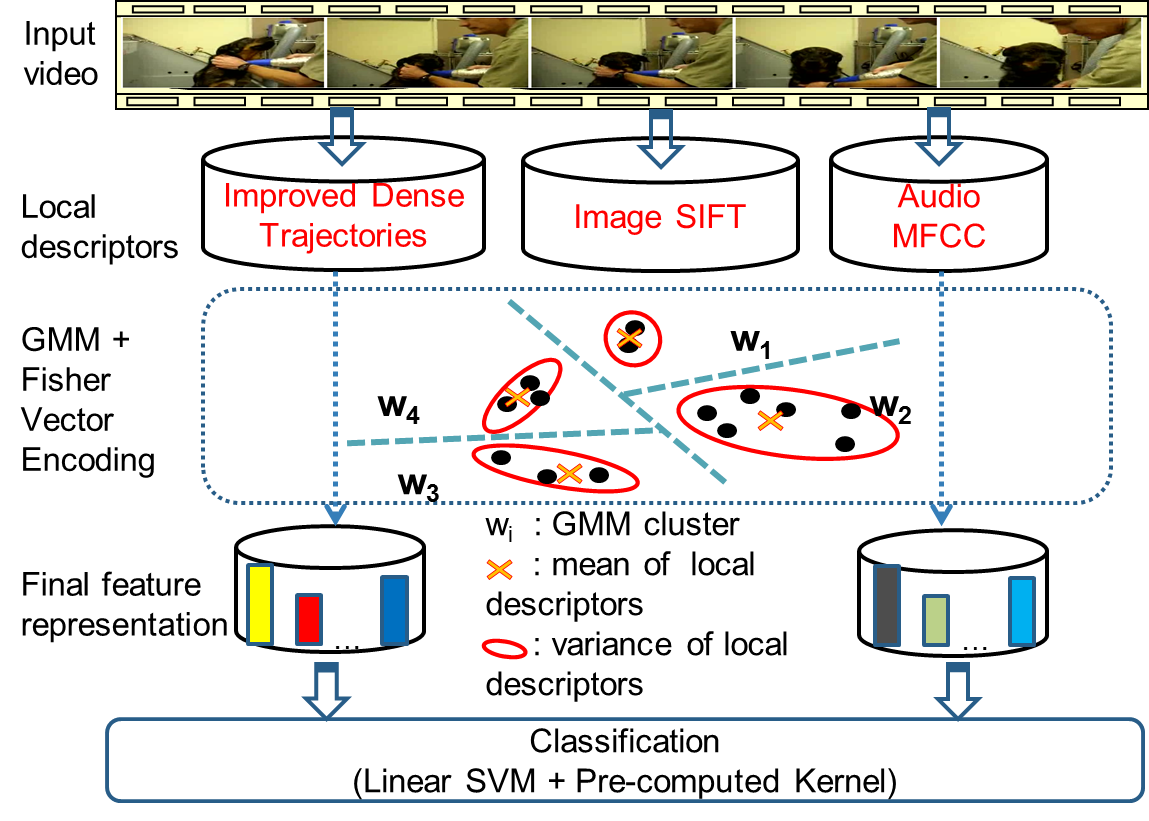
\includegraphics[width=1\linewidth,height=1\linewidth]{Images/framework_fv.png}
	\caption{Our framework for Fisher vector encoding.}
	\label{fig:fv_encoding}
\end{figure*}
Fisher Vector (FV) was first introduced in \cite{jaakkola1999exploiting} for image classification. Fisher vector has also been used in action recognition such as \cite{sun2013large}, \cite{wang2013action}. Fisher vector encoding can be considered as an extension of Bag-of-word encoding. Unlike bag of features, Fisher vector encodes both first and second order statistics between the local descriptors and the codebook. As a result, the length of the Fisher vector is much longer than the length of the BoW feature when using the same codebook. 

Different from bag-of-word encoding, which often employs KMeans to train the codebook. Fisher vector often uses the Gaussian Mixture Model (GMM) to encode the relative position of each local descriptor to each mixture center. Due to the more expressiveness of the Fisher vector, it can achieve a comparable performance with BoW while using a much smaller codebook \cite{sanchez2013image}, \cite{sun2013large}. The pipeline of our Fisher vector framework is shown in Fig. \ref{fig:fv_encoding}.

In our experiment, we set the number of Gaussians in the GMM model to K = 256. Then we randomly select 1,000,000 local descriptors for training the model. As suggested in \cite{perronnin2010improving}, it is better to reduce the local feature dimension using Principal Component Analysis (PCA). Normalization of output feature is also very important for Fisher vector. Following the recommendation in \cite{perronnin2010improving}, we apply power normalization with $\alpha=0.5$, and then L2-normalization to the Fisher vector.

\subsection{Training Violent Classifiers}

%\subsection{Learning Classification}
LibSVM \cite{LibSVM} is used for training and testing at shot level. To generate training data, shots which fall into positive segments more than 80\% will be considered as positive shots. The remaining shots are considered as negative. Extracted features are scaled to [0, 1] using the svm-scale tool of LibSVM. We use $\chi^2$ kernel to calculate the distance matrix. The optimal (C;g) parameters for learning SVM classifiers are found by conducting a grid search with 5-fold cross validation on the original dataset. For features that are encoded using the Fisher vector encoding, we also use LibSVM but with linear kernel. In this case, we also do a 5-fold cross-validation to obtain the learning parameter C.

\subsection{Late Fusion}
Fusing information coming from different media seems a natural way to handle multimedia content. Fusing of multi-modal information has been widely used for tasks including multimedia event detection, video search, etc. Naturally different semantic events, types of multimedia data have their own characteristics so their fusion strategies could be different also. In this evaluation, we simply use the late fusion with average weighting scheme for all features \cite{snoek2005early} because our focus is the performance comparison of features for VSD.

\section{VSD Features}
\label{vsd_feature}

\subsection{Visual Global Features}

We evaluate both global features and local features. We selected the best configuration of each types of features from our previous work\cite{lam2012nii}. The global features include color moments, color histogram, edge orientation histogram, and local binary patterns with different configuration:

\begin{itemize}
	\item Granularity:  Since global features do not capture spatial information, to overcome this problem, a grid n \ding{53} m usually used to divide the input image into non overlapping sub-regions. The features extracted from these regions are concatenated to form the feature vector for the image.
	\item Color space: Local binary patterns (LBP) and edge orientation histogram (EOH) are extracted from gray scale image. For color moments and color histogram, color spaces including HSV, RGB, Luv, and YCrCb are used.
	\item Quantization: For color histogram, we only use 8-bin histogram for each channel. For edge orientation histogram, we quantize orientations into histograms of 36 (edge) + 1(non-edge) bins. For local binary patterns, we quantize binary patterns into histograms of 30, 59 bins.
\end{itemize}

\subsection{Visual Local Features}
\subsubsection{Still Image Feature}

For local feature, we use popular SIFT with both Hessian Laplace interest points \cite{mikolajczyk2002affine} and dense sampling. In both strategies, local features are extracted at multiple scales using the Gaussian scale space \cite{mikolajczyk2002affine}. In case of dense sampling, the key points are sampled densely on a grid with the step size of 6 pixels (dense6mul). One the key point is detected, it is described by the standard SIFT ~\cite{lowe2004distinctive}, RGB-SIFT, Opponent-SIFT and C-SIFT ~\cite{burghouts2009performance}.

\subsubsection{Motion Feature}
As shown by Wang et al. \cite{wang2013action}, Dense Trajectory feature is one of the best approaches for action classification. Dense Trajectory has an efficient solution to remove camera motion. In the Hollywood movies, there are a lot of action with different movie effects in the violent scenes. We apply the dense trajectory to capture these information. Trajectories are obtained by tracking the densely sampled points in the optical flow fields. As it is suggested by Wang \cite{wang2013action}, we use Histogram of Oriented Gradient (HOG), Histogram of Optical Flow (HOF) and Motion Boundary Histogram (MBH) to describe each trajectory. HOG is used to capture appearance characteristics of the moving object while HOF captures the speed of the moving object. The last descriptor, MBH, can capture boundary of the motion and is good for handling camera motion.

\subsubsection{Audio Feature}
We use the popular Mel-frequency Cepstral Coeffcients (MFCC) \cite{rabiner2007introduction} for extracting audio feature. We choose a window size of 25 ms for audio segment and a step size of 10 ms. The 13-dimensional MFCC vectors along with each first and second derivatives are used for representing each audio segment. Raw MFCC features are also encoded using BoW. These configurations are also used by AXES/LEAR team in TRECVID Multimedia Event Detection 2013 \cite{aly2013axes} and THUMOS Challenge 2014 \cite{oneata2014lear} in which they won the best performance.

\subsection{Mid-level Feature}
\subsubsection{VSD Concepts}

Violent scene detection is also a kind of high level recognition task. Violence concept has high semantic meaning and high
variability in appearance. Besides that, due to lack of training data for this concept, training violence classifier directly
from low-level features is not effective. Instead of focusing on selecting the low-level features for VSD, we investigate how to use related violent information as mid-level feature to detect violent scene in the movie. We manually select the violent information which are annotated by human assessors as related attributes of violence concept.Then we propose to use such concepts as related semantic attributes of the original violence concept. Figure \ref{fig:exampleVS} shows how to describe the violent scene by their semantic attributes. These attributes which can be more well-presented by low-level features (e.g. the attribute about ”blood” can be sufficiently presented by color) are used to create the mid-level features. In other words, the attributes have smaller gap to the low-level features, compared to the original violence concept. For example, in Figure 1, because violence occurred during the whole scene, it is very hard to use low-level features to represent the violence concept. But, we can use the low-level visual features to represent some attributes such as “fire”, ”blood”. By doing this, we narrow the semantic gap between the original violence concept and low-level features extracted from video shots.
\begin{figure*}[!t]
	\centering
	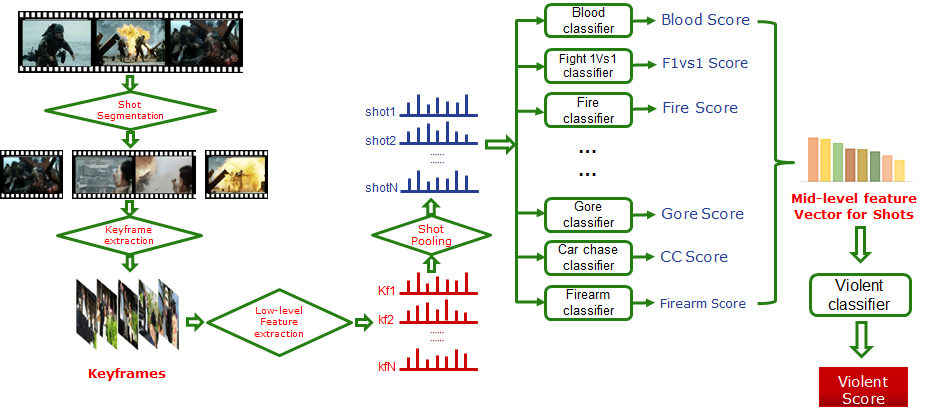
\includegraphics[width=2\linewidth]{Images/Mid-level.png}
	\caption{Overview of Mid-level framework.}
	\label{fig:mid-level}
\end{figure*}
Attributes related to violence concept are manually defined. We used seven related concepts provided in MediaEval Dataset as violent attributes. Our mid-level framework is shown in Figure~\ref{fig:mid-level}. Firstly, each corresponding attribute classifier is trained by using low-level features. Secondly, the mid-level features of a training (or test) video shots are formulated by concatenating scores returned by attribute classifiers. At the moment, we use the same weights for concatenating different scores. Then thirdly, we use this feature to train the mid-level feature-based violence classifier. Finally, we apply this violence classifier on test set to get the violence score for each shot (these shots are also represented by mid-level features).

\subsubsection{Deep Learning Feature}
Mid-level features can also be learnt from out of domain concepts such as ObjectBank \cite{15} or ActionBank \cite{23}. However, learning off-the-shelf concepts is less effective than using shallow methods. Recently, Krizhevsky \cite{krizhevsky2012imagenet} proposed a deep learning framework which significantly outperformed previous state-of-the-art methods on the ImageNet benchmark \cite{deng2009imagenet}. One interesting thing is this deep learning model can be used to extract feature on other benchmarks as an off-the-shelf object detector \cite{donahue2013decaf}. 

In this evaluation, we adopt the popular DeepCaffe \cite{jia2014caffe} framework for extracting keyframe features. We use the pre-trained deep model provided by DeepCaffe. This model was trained on ImageNet 1,000 concepts \cite{deng2009imagenet}. The detail protocol for training the model is described in \cite{jia2014caffe}. As suggested in \cite{krizhevsky2012imagenet}, we select the last three fully-connected layers for feature representation. The third and second to last layer has 4,096 dimension while the last layer has 1,000 dimension corresponding to 1,000 concept categories in the ImageNet dataset.

\section{Experiments}
\subsection{Dataset}
In this paper, we used the dataset from MediaEval  Affect Task 2014 \cite{demarty2014benchmarking}, this is a set of 31 Hollywood movies that must be purchased the original DVD due to copyright issues. The movies are of different genres (from extremely violence movies to movies without violence). In this dataset, we focus on the violent concept with subjective definition, which is defined as “those which one would not let an 8 years old child see because they contain physical violence”. Follow the proposed method, we divide this dataset into 2 parts:

\begin{table}
	\caption{DEVEL set includes 24 Hollywood movies.}
	\setlength{\tabcolsep}{4pt}
%	\renewcommand{\arraystretch}{0.9}
	\begin{tabular}{clccc}
		\hline
		\textbf{No.}         & {\textbf{Video Name}} & {\begin{tabular}[x]{@{}c@{}}\textbf{Length}\\\textbf{(in Seconds)}\end{tabular}} & {\textbf{\#keyframes}} & {\textbf{\#shot}} \\ \hline
			1 & Armageddon & 8,681.05 & 217,026 & 1,737 \\ 
			2 & BillyElliot & 6,349.36 & 158,734 & 1,270 \\
			3 & Eragon & 5,985.57 & 149,639 & 1,198 \\ 
			4 & Harry Potter 5 & 7,954.72 & 198,868 & 1,591 \\
			5 & I Am Legend & 5,780.58 & 144,514 & 1,157 \\ 
			6 & Leon & 6,344.49 & 158,612 & 1,269 \\ 
			7 & Midnight Express & 6,960.96 & 174,024 & 1,393 \\ 
			8 & {\begin{tabular}[x]{@{}c@{}}Pirates Of The\\Caribbean 1\end{tabular}}  & 8,241.01 & 206,025 & 1,649 \\ 
			9 & Reservoir Dogs & 5,712.98 & 142,825 & 1,143 \\ 
			10 & Saving Private Ryan & 9,750.89 & 243,772 & 1,951 \\ 
			11 & The Sixth Sense & 6,178.01 & 154,450 & 1,236 \\ 
			12 & The Wicker Man & 5,870.89 & 146,772 & 1,175 \\ 
			13 & The Bourne Identity & 6,816.29 & 170,407 & 1,364 \\
			14 & The Wizard of Oz & 5,859.29 & 146,482 & 1,172 \\ 
			15 & Dead Poets Society & 7,415.17 & 185,379 & 1,484 \\
			16 & Fight Club & 8,006.34 & 200,158 & 1,602 \\ 
			17 & Independence Day & 8,834.96 & 220,874 & 1,767 \\
			18 & The God Father & 10,194.96 & 254,874 & 2,039 \\ 
			19 & Pulp Fiction & 8,887.97 & 222,199 & 1,778 \\ 
			20 & Forrest Gump & 8,176.97 & 204,424 & 1,636 \\ 
			21 & Fargo & 5,646.34 & 141,158 & 1,130 \\ 
			22 & The Pianist & 8,567.10 & 214,177 & 1,714 \\ 
			23 & Fantastic Four 1 & 6,094.41 & 152,360 & 1,219 \\ 
			24 & Legally Blond & 5,523.49 & 138,087 & 1,105 \\ \hline
			& \textbf{Total} & \textbf{173,833.8} & \textbf{4,345,840} & \textbf{34,779} \\ \hline
	\end{tabular}
	\label{devel-dataset}
\end{table}


\begin{table}
	\caption{TEST set includes 7 Hollywood movies.}
	\setlength{\tabcolsep}{4pt}
%	\renewcommand{\arraystretch}{0.9}
	\begin{tabular}{clccc}
		\hline
		\textbf{No.}         & {\textbf{Video Name}} & {\begin{tabular}[x]{@{}c@{}}\textbf{Length}\\\textbf{(in Seconds)}\end{tabular}} & {\textbf{\#keyframes}} & {\textbf{\#shot}} \\ \hline
		1 & V for Vendetta & 7,626.49 & 190,662 & 1,526 \\ 
		2 & Terminator 2 & 8,831.37 & 220,784 & 1,767 \\ 
		3 & Jumanji Collectors & 5,993.98 & 149,849 & 1,199 \\ 
		4 & Ghost in the Shell & 4,966.00 & 124,150 & 994 \\ 
		5 & Desperado & 6,012.89 & 150,322 & 1,203 \\ 
		6 & Brave Heart & 10,224.49 & 255,612 & 2,045 \\ 
		7 & 8 Mile & 6,355.53 & 158,888 & 1,272 \\ \hline
		  & \textbf{Total} & \textbf{50,010.75} & \textbf{1,250,267} & \textbf{10,006} \\ \hline
	\end{tabular}
	\label{test-dataset}
\end{table}

\begin{itemize}
	\item DEVEL (Table~\ref{devel-dataset}): this is training dataset; used to train violence classifiers; has 24 movies, total 34,779 shots, 48.29 hours. 
	\item TEST (Table~\ref{test-dataset}): this is testing dataset; used to test and evaluate the system; has 7 movies, total 10,006 shots and 13.89 hours.
\end{itemize}
Total duration are about 62.18 hours, with 44,785 shots. To reduce the computation cost, when we extract keyframes, we resize the keyframes to 500x400 pixels.
\subsection{Groundtruth}
By using subjective definition in MediaEval VSD 2014\cite{demarty2014benchmarking}, the ground truth is created by human assessors and provided by the MediaEval organizers. In addition to segments containing physical violence, annotations also include the following high-level concepts: presence of blood, fights, presence of fire, presence of guns, presence of cold arms, car chases and gory scenes, for the visual modality; gunshot, explosion and scream for the audio modality. The ground truth data are provides in segment. To generate training data, we consider the positive shots are the ones which have 80\% overlapping with ground truth segments.
\subsection{Evaluation Metrics}
As evaluation metric, we used MediaEval VSD official metric (MAP2014-mean average precision, 2014 version). This is an adapted version of mean average precision (MAP). The MAP2014 is computed based on the ranked list of shots returned by the detection system and the ground truth provided by the task organizers. Mean average precision for MediaEval VSD  is calculated as below:
\[
MAP=\ \frac{\sum_{v=1}^VAP(v)}{V},
\]
where V is number of test videos and AP is average precision for each video. MediaEval VSD Organizers define the average precision measure as follows: all segments marked as violent by the algorithm under consideration are sorted in descending order, according to the given confidence scores. An algorithm’s prediction of violence is considered a hit if the predicted segment overlaps with the corresponding ground truth segment by more than 50\% (or the other way round). To counteract the above mentioned problem when predicting many short segments, several hits on the same ground truth segment only count as one true positive. The others are ignored, thus not counted as false positives either.
\subsection{Results and Comparisons}
\subsubsection{Global Features}
\begin{table}
	\centering
	\caption{Comparison of visual global features, sorted by MAP2014.}
	\setlength{\tabcolsep}{4pt}
	\begin{tabular}{llcccc}
		%\toprule
		\hline
		Features & Color space & Quantization & MAP2014(\%) \\ \hline
		%\midrule
		LBP & GRAY  & 59    & 31.18 \\
		EOH & GRAY   & 36    & 24.20 \\
		CH & RGB   & 8x3   & 23.53 \\
		CM & HSV     & 3x3   & 22.21 \\
		CM & Luv      & 3x3   & 21.68 \\
		CH & Luv    & 8x3   & 21.56 \\
		CH & HSV    & 8x3   & 20.73  \\
		CM & RGB     & 3x3   & 20.17 \\
		CM & YCrCb   & 3x3   & 17.81 \\
		CH & YCrCb   & 8x3   & 17.79 \\ \hline
		%\bottomrule
	\end{tabular}%
	\label{tab:global}%
\end{table}%

Performance of global image features is shown in Table \ref{tab:global}. Among evaluated global feature, LBP has the best performance, followed by EOH. Performance of color features such as CH and CM generally lower than EOH and LBP even with different grid configurations. Color information is useful for violent detection especially when there is presence of color-specific concepts such as blood in the movie. However, their presences might be too short which make it difficult to retain after the keyframe sampling step.

On the other hand, color information can be confusing when one single concept has multiple-colored appearances. For example, the concept of fire can come with red, or white, or even blue color. In these cases, capturing the appearance information such as edge is more useful. That can be why EOH has stronger performance than color features. 

LBP often captures more information than EOH. It can also utilize the texture characteristics of the image in the feature representation. These texture pattern can be typical in violent scenes such as car chase and war scenes. That is why the performance of LBP is far better than the remaining global features.
\subsubsection{Local Features}

\begin{table}
	\centering
	\caption{Comparison of visual local features using BoW encoding, sorted by MAP2014.}
	\begin{tabular}{llccc}
		%\toprule
		\hline
		Keypoint descriptor & Keypoint detector & MAP2014(\%) \\ \hline
		%\midrule
		RGB\_SIFT & Densampling & 46.56 \\
		SIFT  & Densampling & 41.85 \\
		SIFT  & Harlap & 41.49 \\
		RGB\_SIFT & Harlap & 40.67 \\
		Opponent\_SIFT & Densampling  & 34.29 \\
		Color\_SIFT & Densampling  & 34.22 \\
		Opponent\_SIFT & Harlap & 31.38 \\
		Color\_SIFT & Harlap & 30.13 \\ \hline
		%\bottomrule
	\end{tabular}%
	\label{tab:local}%
\end{table}%
Performance evaluation of local image features is shown in Table \ref{tab:local}. At first, we extensively compare two keypoint extraction methods: one using Harlap operator and one using dense sampling strategy. Both of types were extracted at six different scales. Experimental results show that dense sampling strategy always outperforms Harlap keypoint detector. This observation is also same with what was reported in \cite{bosch2006scene} and \cite{bosch2007image}.

In general SIFT features with color information have stronger performance for VSD. Among color SIFT features, RGB-SIFT has the best performance in both cases: with and without using spatial configuration. However, using the standard SIFT can already get a reasonably good performance, considering to its efficiency. 

%When spatial information is used, the performance is significantly improved. For example, performance of RGB-SIFT increases from 38.86 \%  to 42.08 \% when using the grid of 3x1 and to 45.06 \% when grid of 2x2 is applied. We also observe the same performance improvement in other types of SIFT features when spatial information is encoded. In most cases, using the grid of 2x2 returns a better performance. 

\subsubsection{Motion Features}
Performance evaluation of local image features is shown in Table \ref{tab:motion_bow}. Basically, we compare different types of descriptors for trajectory-based features. In term of single trajectories descriptor, MBH leads to a better performance. The reason can be due to its robustness in reducing camera motion which often appears in action movies. The performance of HOG/HOF descriptor is much weaker than MBH, which is also confirmed in \cite{wang2013action}. That is why their combination using the average weight of late fusion does not help improve the performance.
\begin{table}
	\centering
	\caption{Comparison of motion descriptors for the improved dense trajectories feature using the BoW encoding, sorted by MAP2014.}
	\begin{tabular}{lccc}
		%\toprule
		\hline
		Descriptor & MAP2014(\%) \\ \hline
		%\midrule
		MBH   & 48.15 \\
		HoG\_HoF\_MBH & 46.52 \\
		HoG\_HoF & 42.22 \\ \hline
		%\bottomrule
	\end{tabular}%
	\label{tab:motion_bow}%
\end{table}%

\subsubsection{Comparison Between BoW and FV}
It is well-known that Fisher vector is more efficient and effective than the tradional bag-of-words model for different visual recognition task. In this evaluation, we also conduct experiments to see whether FV can help for VSD. There representative features from there modalities: visual motion, visual image and audio were selected for the comparison. The results of these experiments are shown in Table \ref{tab:bow_fv}. FV vector does help improve the performance of visual features. The performance gain of motion features is larger than that of image feature. However, FV seems to be not effective for audio feature.

\begin{table*}[htbp]
	\centering
	\caption{Performance comparison of Bag-of-words and Fisher vector encoding.}
	\begin{tabular}{lcccc}
		\hline
		szFeature & BoW(\%) & FV(\%) \\ \hline
		Motion feature (Densetrajectories + HOGHOFMBH) & 46.52 & 50.77 \\
		Local features (SIFT + Dense6mul) & 33.82 & 29.21 \\
		Audio feature (MFCC) & 28.32 & 28.32 \\ \hline
	\end{tabular}%
	\label{tab:bow_fv}%
\end{table*}%

\subsubsection{Mid-level Feature}
\begin{table}
	\centering
	\caption{Comparison of in-domain and out-domain of mid-level features, sorted by MAP2014.}
	\begin{tabular}{lcc}
		%\toprule
		\hline
		Feature & MAP2014(\%) \\ \hline
		VSD	attributes & 34.99 \\ \hline
		%\midrule
		\textbf{Deep feature (layer 7)} &\textbf{ 48.33} \\
		Deep feature (layer 6) & 41.78 \\
		Deep feature (layer 8) & 33.80 \\ \hline
		%\bottomrule
	\end{tabular}%
	\label{tab:midlevel}%
\end{table}%
We report the performance comparison of using mid-level feature for VSD in Table \ref{tab:midlevel}. The VSD attributes represent for in-domain mid-level features because these attribute detectors were trained on VSD data. On the other hand, deep features were trained on out-of-domain data, in this case, ImageNet dataset.

The performance of VSD attributes is slightly better than Deep feature at layer 8. This is an interesting result given knowing that deep feature at layer 8 is a 1,000-dimensional vector compared to 13-dimensional vector of VSD attributes. This result demonstrates that using the in-domain data is very important there is still a big gap when adapting feature from out-of-domain data.

However, this gap can be overcome when using deep feature at hidden layers. As observed in Table \ref{tab:midlevel}, using deep feature at layer 6 and 7 significantly improves the performance. This is because deep feature at fully connected hidden layers captures richer information than the last layer \cite{donahue2013decaf}. The performance of layer 6 or layer 7 can depend on the specific task. For VSD, we recommend using layer 7 to obtain the best performance.

\subsubsection{Best of Each Feature Types}
In Table \ref{tab:summary}, we summarize the performance of each feature type for VSD. Motion features and deep learning features are among the best single feature for MED. The reason is due to the fact that in VSD movies, there are a lot of motion clues that can be very informative to detect violent scene. Moreover, deep learning feature can give a richer representation for images. That is why it has better performance compared to other local or global feature extraction methods. Audio feature itself does not provide reasonably good accuracy for recognizing violence. However, it can be complementary when combining which other features. 

In the bottom half of Table \ref{tab:summary}, we also present the performance comparison when combining different features together. If we combine all features together, the performance is lower than the best one. So this is not a good strategy and it is important to select which features to combine. In the second experiment, we only select the best performing features that is shown in the first half of Table \ref{tab:summary} for combining (for global features: LBP, for local featurse: RGB\_SIFT, for motion features: HoG\_HoF\_MBH with fisher vector encoding, for audio features: MFCC, for mid-level features: Deep feature with out-domain concepts from IMAGENET). The performance of this case in much better with around 2\% improvement compared to the best one. We further select a subset of best features for fusion. We found that, the combination of motion, deep feature, audio and local image feature performs the best. Therefore, we recommend using this fusion strategy for a better VSD system.

\begin{table}
	\centering
	\caption{Summary of performance of each feature and their combination using late fusion.}
	\begin{tabular}{lcc}
		\hline
		Feature types & MAP2014(\%) \\ \hline
		Motion (FV) & 50.77 \\
		Deep feature & 48.33 \\
		Local & 46.56 \\
		VSD Attribute & 34.99 \\
		Global & 31.18 \\
		Audio & 28.32 \\  \hline
		\textbf{Local + Motion + Deep + Audio} & \textbf{56.41} \\
		All best single features & 52.52 \\
		All features & 45.99 \\ \hline
	%	All locals (BoW) & 0.44155 & 0.677429 \\ \hline
	\end{tabular}%
	\label{tab:summary}%
\end{table}%
Example of violent scenes detected by our best system is shown in Fig. \ref{fig:bestdemo}. A yellow face represents a correct detection while a green face represents an incorrect one. Our best system can detect many correct violent scenes with high confidence. The shot in the 8th row is a false positive one. In this case, this is a scene about a car chase. However, the is no fatalities or injures in this scene. Therefore, it is still not considered as a violent scene according the violent scene's definition. This is a very sensitive case, which is very difficult to differentiate even for human. 

\begin{figure*}
	\centering
	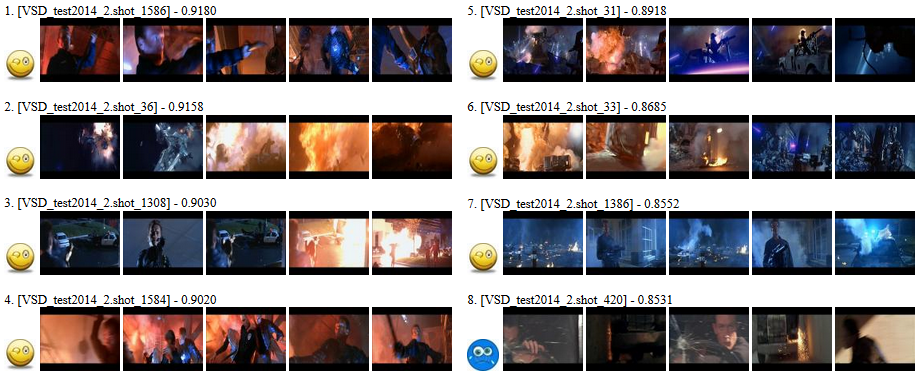
\includegraphics[width=2\linewidth]{Images/BestRun_shot8th_CarChase_NoInjure.png}
	\caption{Example of violent scenes detected by our best system. This figure is best viewed in color.}
	\label{fig:bestdemo}
\end{figure*}

\subsubsection{Comparison with Other MediaEval Teams}

Finally, we compare the performance of our VSD system with other systems submitted to the VSD Challenge in 2014. The performance of each team is 
shown in Table \ref{tab:mediaeval}. According to the official result released by MediaEval's organizer, our system achieved the runner-up performance, only lower than the system of Fudan University \cite{2014fudan}. It is worth noted that Fudan University used a score smoothing techniques to improve the final MAP. In our case, we did not apply any post-processing technique onto the rank list. The best result of Fudan University without using post-processing is 51.4 \% in terms of MAP2014. Therefore, technically, our system can achieve better performance than Fudan University when post-processing is not applied. 

Comparing to the remaining teams, our system achieved a much stronger performance. For example, our performance is higher than the third team up to 22\% (relatively) \cite{2014far}. The reason can be due to they only use audio feature in their best run. In general, our VSD system has already become a state-of-the-art sytem for detecting violent scenes in movies.
\begin{table}
	\centering
	\caption{Comparison with MediaEval teams, sorted by MAP2014.}
	\begin{tabular}{lcc}
		\hline
		MediaEval VSD Team & MAP2014(\%) \\ \hline
		Fudan \cite{2014fudan} & 63.0 \\
		\textbf{NII-UIT} \cite{2014nii} (\textbf{Ours}) & \textbf{56.4} \\
		FAR \cite{2014far} & 45.1 \\
		MIC-TJU \cite{2014mic} & 44.6 \\
		Recod \cite{avila2014recod} & 37.6 \\
		VIVOLAB \cite{2014vivolab} & 17.8 \\
		TUB-IRML \cite{2014tub} & 17.2 \\
		MTMDCC \cite{2014mtm} & 2.6 \\ \hline
	\end{tabular}%
	\label{tab:mediaeval}%
\end{table}%
\subsubsection{Summary of Evaluation}
The definition of violent scene can be involved with multiple objects, scenes and actions.  Experimental results show that still features can detect static violent scenes such as blood, fire and explosion. Audio features achieve reasonable performance when there are gun sounds, fighting or fast-moving objects in the action movies. However, many false positives are also detected because some scenes are not considered as violent scenes even though they contain the same audio information.  
Violent movies often contain a number of violent actions such as fighting, chasing and slaughter.  Therefore, motion features can achieve better detection performance than others. However, because VSD is a multimedia problem, it is necessary to combine with other features as well.
Due to the large diversity of the violent concepts, it is almost impractical to use in-domain VSD concepts.  In this evaluation, we also use 7 VSD concepts with only around dozens of annotated segments for each concept.  Expanding the number of in-domain can increase the performance but it is a costly approach.  On the other hand, we show that using a large number of out-of-domain concepts which are represented by deep learning features can also gain a substantial improvement.

\section{Discussion and Conclusion}
We evaluated the performance of various features for the violent scene detection. The features that were evaluated include global, local image feature, motion feature, audio feature, VSD concept feature and deep learning feature. We also compare the two popular encoding strategy: bag-of-words and Fisher vector. In term of single feature performance, motion feature is very good for VSD. This highest performance was obtained when using with the Fisher vector encoding. The performance of deep learning feature extracted at the second-to-last fully connected layer is also reasonably good. This result appeals the application of deep learning for VSD.   

We can even get better results when combining these evaluated features together. However, as shown in our experiments, combining all features in simple way (e.g. average fusion) is not effective. The correct way to combine is to only select the best performing feature from each type of features. We can also achieve a higher performance when carefully select which type of features to combine. To this end, we recommend combining local image feature, motion feature, audio feature and deep learning feature to obtain the best performance for VSD.

In terms of system comparison without using post-processing, comparing with other participants on the MediaEval 2014 VSD benchmark, we are one of the best systems. Therefore our technologies is state-of-the-art, and our study can be served as a good reference for other researchers who want to build violent scene detection systems. 

%%%%%%%%%%%%%%%%%%%%%%%%%%%%%%%%%%%%%%%%%%%%%%
%%                                          %%
%% Backmatter begins here                   %%
%%                                          %%
%%%%%%%%%%%%%%%%%%%%%%%%%%%%%%%%%%%%%%%%%%%%%%

\begin{backmatter}

\section{Acknowledgements}
This research is funded by Vietnam National University Ho Chi Minh City (VNU-HCM) under grant number B2013-26-01.

%%%%%%%%%%%%%%%%%%%%%%%%%%%%%%%%%%%%%%%%%%%%%%%%%%%%%%%%%%%%%
%%                  The Bibliography                       %%
%%                                                         %%
%%  Bmc_mathpys.bst  will be used to                       %%
%%  create a .BBL file for submission.                     %%
%%  After submission of the .TEX file,                     %%
%%  you will be prompted to submit your .BBL file.         %%
%%                                                         %%
%%                                                         %%
%%  Note that the displayed Bibliography will not          %%
%%  necessarily be rendered by Latex exactly as specified  %%
%%  in the online Instructions for Authors.                %%
%%                                                         %%
%%%%%%%%%%%%%%%%%%%%%%%%%%%%%%%%%%%%%%%%%%%%%%%%%%%%%%%%%%%%%

% if your bibliography is in bibtex format, use those commands:
\bibliographystyle{bmc-mathphys} % Style BST file
\bibliography{mybibfile}      % Bibliography file (usually '*.bib' )

% or include bibliography directly:
% \begin{thebibliography}
% \bibitem{b1}
% \end{thebibliography}

%%%%%%%%%%%%%%%%%%%%%%%%%%%%%%%%%%%
%%                               %%
%% Figures                       %%
%%                               %%
%% NB: this is for captions and  %%
%% Titles. All graphics must be  %%
%% submitted separately and NOT  %%
%% included in the Tex document  %%
%%                               %%
%%%%%%%%%%%%%%%%%%%%%%%%%%%%%%%%%%%

%%
%% Do not use \listoffigures as most will included as separate files


%%%%%%%%%%%%%%%%%%%%%%%%%%%%%%%%%%%
%%                               %%
%% Tables                        %%
%%                               %%
%%%%%%%%%%%%%%%%%%%%%%%%%%%%%%%%%%%

%% Use of \listoftables is discouraged.
%%

\end{backmatter}
\end{document}
